\chapter{ТЕОРЕТИЧНІ ЗАСАДИ ПІДВИЩЕННЯ ЕФЕКТИВНОСТІ ПОШУКУ (ДОСЛІДЖЕННЯ) ПОТЕНЦІЙНО-НЕБЕЗПЕЧНИХ ДЕФЕКТІВ ПРОЕКТУВАННЯ ТА РЕАЛІЗАЦІЇ ЦІЛЬОВИХ ПРОГРАМ}
\label{2section::doc}\label{2section:id1}

%TODO зкоротити опис метрик


\section{Інтегровані властивості цільової програми}
\label{2section:id2}
На відміну від більшості галузей матеріального виробництва, в питаннях проектів створення ПЗ неприпустимі прості підходи, засновані на множенні трудомісткості на середню продуктивність праці. Це викликано, насамперед, тим, що економічні показники проекту нелінійно залежать від обсягу робіт, а при обчисленні трудомісткості допускається велика похибка.

Тому для вирішення цього завдання використовуються комплексні і досить складні методики, які вимагають високої відповідальності в застосуванні і певного часу на адаптацію (настройку коефіцієнтів).

Сучасні комплексні системи оцінки характеристик проектів створення ПЗ можуть бути використані для вирішення наступних завдань:
\begin{itemize}
\item {} 
попередня, постійна і підсумкова оцінка економічних параметрів проекту: трудомісткість, тривалість, вартість;

\item {} 
оцінка ризиків по проекту: ризик порушення строків та невиконання проекту, ризик збільшення трудомісткості на етапах налагодження та супроводження проекту та пр;

\item {} 
прийняття оперативних управлінських рішень - на основі відстеження певних метрик проекту можна своєчасно попередити виникнення небажаних ситуацій і усунути наслідки непродуманих проектних рішень.

\end{itemize}


\subsection{Метрики}
\label{2section:id3}
Якість ПЗ - це сукупність властивостей, які визначають корисність вироби (програми) для користувачів відповідно з функціональним призначенням і пред'явленими вимогами .
Характеристика якості програми - поняття, що відображає окремі фактори, що впливають на якість програм і піддаються виміру .

Критерій якості - чисельний показник, що характеризує ступінь, в якій програмі притаманне оцінювана властивість .

Критерії якості включають такі характеристики: економічність, документованість, гнучкість, модульність, надійність, обгрунтованість, тестовані, ясність, точність, модифицируемость, ефективність, легкість супроводу і т.д.

Критерій повинен :
\begin{itemize}
\item {} 
Чисельно характеризувати основну цільову функцію програми ;

\item {} 
Забезпечувати можливість визначення витрат, необхідних для досягнення необхідного рівня якості, а також ступеня впливу на показник якості різних зовнішніх факторів;

\item {} 
Бути по можливості простим, добре вимірним і мати малу дисперсію .

\end{itemize}

Для вимірювання характеристик і критеріїв якості використовують метрики .

Метрика якості програм - система вимірювань якості програм . Ці виміри можуть проводитися на рівні критеріїв якості програм або на рівні окремих характеристик якості. У першому випадку система вимірювань дозволяє безпосередньо порівнювати програми за якістю. При цьому самі виміри не можуть бути проведені без суб'єктивних оцінок властивостей програм. У другому випадку вимірювання характеристик можна виконати об'єктивно і достовірно, але оцінка якості ПЗ в цілому буде пов'язана з суб'єктивною інтерпретацією одержуваних оцінок.

У дослідженні метрик ПО розрізняють два основних напрямки:
\begin{quote}
\begin{itemize}
\item {} 
Пошук метрик, що характеризують найбільш специфічні властивості програм, тобто метрик оцінки самого ПЗ;

\item {} 
Використання метрик для оцінки технічних характеристик і факторів розробки програм, тобто метрик оцінки умов розробки програм.

\end{itemize}

По виду інформації, одержуваної при оцінці якості ПО метрики можна розбити на три групи:
\begin{itemize}
\item {} 
Метрики, що оцінюють відхилення від норми характеристик вихідних проектних матеріалів . Вони встановлюють повноту заданих технічних характеристик вихідного коду.

\item {} 
Метрики, що дозволяють прогнозувати якість розроблюваного ПЗ. Вони задані на безлічі можливих варіантів рішень поставленого завдання і їх реалізації і визначають якість ПЗ, яке буде досягнуто в результаті.

\item {} 
Метрики, за якими приймається рішення про відповідність кінцевого ПО заданим вимогам . Вони дозволяють оцінити відповідність розробки заданим вимогам .

\end{itemize}
\end{quote}


\subsection{ОСНОВНІ НАПРЯМКИ ЗАСТОСУВАННЯ МЕТРИК}
\label{2section:id4}
В даний час у світовій практиці використовується кілька сотень метрик програм. Існуючі якісні оцінки програм можна згрупувати по шести напрямках :
\begin{itemize}
\item {} 
Оцінки топологічної та інформаційної складності програм;

\item {} 
Оцінки надійності програмних систем, що дозволяють прогнозувати отказовие ситуації ;

\item {} 
Оцінки продуктивності ПО і підвищення його ефективності шляхом виявлення помилок проектування ;

\item {} 
Оцінки рівня мовних засобів і їх застосування;

\item {} 
Оцінки труднощі сприйняття і розуміння програмних текстів, орієнтовані на психологічні фактори, суттєві для супроводу і модифікації програм;

\item {} 
Оцінки продуктивності праці програмістів для прогнозування термінів розробки програм і планування робіт зі створення програмних комплексів.

\end{itemize}


\subsection{МЕТРИЧНІ ШКАЛИ}
\label{2section:id5}
Залежно від характеристик і особливостей застосовуваних метрик їм ставляться у відповідність різні вимірювальні шкали.

Номінальною шкалою відповідають метрики, що класифікують програми на типи за ознакою наявності або відсутності деякої характеристики без урахування градацій.

Порядкової шкалою відповідають метрики, що дозволяють ранжувати деякий характеристики шляхом порівняння з опорними значеннями, тобто вимір за цією шкалою фактично визначає взаємне положення конкретних програм.

Інтервального шкалою відповідають метрики, які показують не тільки відносне положення програм, але і те, як далеко вони відстоять один від одного.

Відносній шкалі відповідають метрики, що дозволяють не тільки розташувати програми певним чином і оцінити їх положення відносно один одного, а й визначити, як далеко оцінки відстоять від кордону, починаючи з якої характеристика може бути виміряна.

Метрика СКЛАДНОСТІ ПРОГРАМ
\begin{description}
\item[{При оцінці складності програм, як правило, виділяють три основні групи метрик :}] \leavevmode\begin{itemize}
\item {} 
Метрики розміру програм

\item {} 
Метрики складності потоку управління програм

\item {} 
І метрики складності потоку даних програм

\end{itemize}

\end{description}

.
Метрика РОЗМІРУ ПРОГРАМ.

Оцінки першої групи найбільш прості і, очевидно, тому отримали широке поширення. Традиційною характеристикою розміру програм є кількість рядків вихідного тексту. Під рядком розуміється будь-який оператор програми, оскільки саме оператор, а не окремо взята рядок є тим інтелектуальним '' квантом '' програми, спираючись на який можна будувати метрики складності її створення.
Безпосереднє вимірювання розміру програми, незважаючи на свою простоту, дає хороші результати. Звичайно, оцінка розміру програми недостатня для прийняття рішення про її складності, але цілком застосовна для класифікації програм, істотно різняться обсягами. При зменшенні відмінностей в обсязі програм на перший план висуваються оцінки інших факторів, що впливають на складність . Таким чином, оцінка розміру програми є оцінка за номінальною шкалою, на основі якої визначаються тільки категорії програм без уточнення оцінки для кожної категорії .

До групи оцінок розміру програм можна віднести також і метрику Холстеда .
\begin{description}
\item[{МЕТРИКА Холстеда .}] \leavevmode
Основу метрики Холстеда складають чотири вимірюваних характеристики програми :
n1 - число унікальних операторів програми, включаючи символи -
роздільники, імена процедур і знаки операцій ( словник операторів ) ;
n2 - число унікальних операндів програми ( словник операндів ) ;
N1 - загальне число операторів в програмі ;
N2 - загальне число операндів в програмі.
Спираючись на ці характеристики, одержувані безпосередньо при аналізі вихідних текстів програм, М. Холстед вводить такі оцінки:

словник програми

n1 = n1 + n2,
довжину програми
N = N1 + N2, ( 1 )
обсяг програми
V = N * log2 ( n ) ( біт). ( 2 )
Під бітом мається на увазі логічна одиниця інформації - символ, оператор, операнд .
Далі М. Холстед вводить n * - теоретичний словник програми, тобто словниковий запас, необхідний для написання програми, з урахуванням того, що необхідна функція вже реалізована в даній мові і, отже, програма зводиться до виклику цієї функції. Наприклад, згідно М. Холстеду, можливе здійснення процедури виділення простого числа могло б виглядати так :

CALL SIMPLE ( X, Y ),
де Y - масив чисельних значень, що містить шукане число X.
Теоретичний словник в цьому випадку буде складатися з
n1 * : \{ CALL, SIMPLE (...) \},
n1 * = 2 ; n2 * : \{ X, Y \},
n2 * = 2,

n * = n1 * + n2 *,
буде дорівнювати 4 .
Використовуючи n *, Холстед вводить оцінку V * :
V * = n ** log2 n *, ( 3 )
за допомогою якої описується потенційний обсяг програми, відповідний максимально компактному тексту програми, що реалізує даний алгоритм .

\end{description}

МЕТРИКА СКЛАДНОСТІ ПОТОКУ УПРАВЛІННЯ ПРОГРАМ.
\begin{quote}

Друга найбільш представницька група оцінок складності програм - метрики складності потоку керування програм. Як правило, за допомогою цих оцінок оперують або щільністю керуючих переходів усередині програм, або взаємозв'язками цих переходів .

І в тому і в іншому випадку стало традиційним уявлення програм у вигляді керуючого орієнтованого графа G = (V, E), де V - вершини, відповідні операторам, а E - дуги, відповідні переходам .

МЕТРИКА МакКейб .
Вперше графічне представлення програм було запропоновано МакКейб . Основний метрикою складності він пропонує вважати цикломатическая складність графа програми, або, як її ще називають, цикломатичне число МакКейб, що характеризує трудомісткість тестування програми .
Для обчислення цикломатическая числа МакКейб Z (G ) застосовується формула

Z ( G) = e - v +2 p,
де e - число дуг орієнтованого графа G ;
v - число вершин ;
p - число компонентів зв'язності графа.
Число компонентів зв'язності графа можна розглядати як кількість дуг, які необхідно додати для перетворення графа в сильно зв'язний . Сильний зв'язковим називається граф, будь-які дві вершини якого взаємно досяжні. Для графів коректних програм, тобто графів, що не мають недосяжних від точки входу ділянок і '' висячих '' точок входу і виходу, сильно зв'язний граф, як правило, виходить шляхом замикання дугою вершини, що позначає кінець програми, на вершину, що позначає точку входу в цю програму.

По суті Z (G ) визначає число лінійно незалежних контурів у Сильно зв'язкового графі . Інакше кажучи, цикломатичне число МакКейб показує необхідну кількість проходів для покриття всіх контурів сильно зв'язного графа або кількість тестових прогонів програми, необхідних для вичерпного тестування за критерієм '' працює кожна гілка'' .

Для програми, граф якої зображений на рис.1, цикломатичне число при e = 10, v = 8, p = 1 визначиться як Z ( G) = 10-8 +2 = 4 .

Цикломатичне число залежить тільки від кількості предикатів, складність яких при цьому не враховується. Наприклад, є два оператора умови:

IF X \textgreater{} 0
THEN X = A ;
ELSE ;
і
IF ( X \textgreater{} 0 \& FLAG = `1 `B ) !
( X = 0 \& FLAG = `0 `B )
THEN X = A ;
ELSE ;
Обидва оператора припускають єдине розгалуження і можуть бути представлені одним і тим же графом (рис. 2 ) . Очевидно, цикломатичне число буде для обох операторів однаковим, що не відображає складності предикатів, що досить істотно при оцінці програм.
\end{quote}
\begin{description}
\item[{МЕТРИКА Майерс .}] \leavevmode
Виходячи з цього Г. Майерс запропонував розширення цієї метрики . Суть підходу Г. Майерса полягає в представленні метрики складності програм у вигляді інтервалу {[}Z (G), Z ( G) + h {]} . Для простого предиката h = 0, а для n -місних предикатів h = n - 1 . Таким чином, перший оператору відповідає інтервал {[} 2,2 {]}, а другий - {[} 2,6 {]} .
По ідеї така метрика дозволяє розрізняти програми, представлені однаковими графами. На жаль, інформація про результати використання цього методу відсутня, тому нічого не можна сказати про його застосовності .

МЕТРИКА ПІДРАХУНКУ точок перетину.
Розглянемо метрику складності програм, що отримала назву '' підрахунок точок перетину '', авторами якої є М. Вудвард, М. Хенель і Д. Хидли . Метрика орієнтована на аналіз програм, при створенні яких використовувалося неструктурні кодування на таких мовах, як мова асемблера і Фортран .
У графі програми, де кожному оператору відповідає вершина, тобто не виключені лінійні ділянки, при передачі управління від вершини a до b номер оператора a дорівнює min ( a, b ), а номер оператора b - max ( a, b ) . Точка перетину дуг з'являється, якщо

min ( a, b ) \textless{} min ( p, q ) \textless{} max ( a, b ) \& max ( p, q ) \textgreater{} max ( a, b ) \textbar{}
min ( a, b ) \textless{} max ( p, q ) \textless{} max ( a, b ) \& min ( p, q ) \textless{} min ( a, b ) .
Іншими словами, точка перетину дуг виникає у разі виходу управління за межі пари вершин ( a, b ) (рис. 3 ) .
Кількість точок перетину дуг графа програми дає характеристики не структурованості програми .

\item[{МЕТРИКА Джілбі .}] \leavevmode
Однією з найбільш простих, але, як показує практика, досить ефективних оцінок складності програм є метрика Т. Джілбі, в якій логічна складність програми визначається як насиченість програми виразами типу IF- THEN - ELSE . При цьому вводяться дві характеристики : CL - абсолютна складність програми, що характеризується кількістю операторів умови; cl - відносна складність програми, що характеризується насиченістю програми операторами умови, тобто cl визначається як відношення CL до загального числа операторів.
Використовуючи метрику Джілбі, ми доповнили її ще однією складовою, а саме характеристикою максимального рівня вкладеності оператора CLI, що дозволило не тільки уточнити аналіз по операторам типу IF- THEN - ELSE, але й успішно застосувати метрику Джілбі до аналізу циклічних конструкцій.

\item[{МЕТРИКА ГРАНИЧНИХ ЗНАЧЕНЬ}] \leavevmode
Великий інтерес представляє оцінка складності програм за методом граничних значень .
Введемо кілька додаткових понять, пов'язаних з графом програми .

Нехай G = (V, E) - орієнтований граф програми з єдиною початковою і єдиною кінцевою вершинами. У цьому графі число входять вершин у дуг називається негативною ступенем вершини, а число що виходять з вершини дуг - позитивної ступенем вершини . Тоді набір вершин графа можна розбити на дві групи: вершини, у яких позитивна ступінь \textless{}= 1 ; вершини, у яких позитивна ступінь \textgreater{} = 2 .

Вершини першої групи назвемо приймаючими вершинами, а вершини другої групи - вершинами відбору.

Для отримання оцінки за методом граничних значень необхідно розбити граф G на максимальне число подграфов G `, що задовольняють таким умовам: вхід в подграф здійснюється тільки через вершину відбору; кожен подграф включає вершину ( звану надалі нижньою межею подграфа ), в яку можна потрапити з будь іншої вершини подграфа . Наприклад, вершина відбору, поєднана сама з собою дугою - петлею, утворює подграф . (рис. 4, таблиця 1 ) .

Число вершин, що утворюють такий подграф, одно скоригованої складності вершини відбору ( таблиця 2 ) . Кожна приймаюча вершина має скориговану складність, рівну 1, крім кінцевої вершини, скоригована складність якої дорівнює 0 . Скориговані складності всіх вершин графа G підсумовуються, утворюючи абсолютну граничну складність програми . Після цього визначається відносна гранична складність програми :

S0 = 1 - ( v - 1 ) / Sa,
де S0 - відносна гранична складність програми ; Sa - абсолютна гранична складність програми ; v - загальне число вершин графа програми .

\item[{Метрика СКЛАДНОСТІ ПОТОКУ ДАНИХ .}] \leavevmode
Інша група метрик складності програм - метрики складності потоку даних, тобто використання, конфігурації і розміщення даних в програмах.
МЕТРИКА ОБІГУ до глобальних змінних .
Розглянемо метрику, що зв'язує складність програм із зверненнями до глобальних змінних .
Пара '' модуль - глобальна змінна'' позначається як ( p, r ), де p - модуль, що має доступ до глобальної змінної r . Залежно від наявності в програмі реального обігу до змінної r формуються два типи пар '' модуль - глобальна змінна'' : фактичні і можливі . Можливе звернення до r за допомогою p показує, що область існування r включає в себе p .

Характеристика Aup говорить про те, скільки разів модулі Up дійсно отримували доступ до глобальних змінних, а число Pup - скільки разів вони могли б отримати доступ.

Відношення числа фактичних звернень до можливих визначається

%Rup = Aup / Pup


Ця формула показує наближену ймовірність посилання довільного модуля на довільну глобальну змінну. Очевидно, чим вище ця вірогідність, тим вище ймовірність несанкціонованої зміни якої-небудь змінної, що може істотно ускладнити роботи, пов\dq язані з модифікацією програми. На жаль, поки не можна сказати, наскільки зручний і точний цей метод на практиці, так як немає відповідних статистичних даних.

\item[{МЕТРИКА Спен}] \leavevmode
Визначення Спен грунтується на локалізації звернень до даних всередині кожної програмної секції. Спен - це число тверджень, які містять даний ідентифікатор, між його першим і останнім появою в тексті програми . Отже, ідентифікатор, що з'явився n раз, має Спен, рівний n - 1 . При великому Спен ускладнюється тестування і налагодження .
1

\item[{МЕТРИКА ЧEПІНА .}] \leavevmode
Суть методу полягає в оцінці інформаційної міцності окремо взятого програмного модуля за допомогою аналізу характеру використання змінних зі списку вводу-виводу.
Всі безліч змінних, складових список введення-виведення, розбивається на 4 функціональні групи:

1 . P - що вводяться змінні для розрахунків та для забезпечення виведення .

Прикладом може служити використовувана в програмах лексичного аналізатора змінна, що містить рядок вихідного тексту програми, тобто сама змінна не модифікується, а лише містить вихідну інформацію .

2 . M - модифікуються, або створювані всередині програми змінні.

3 . C - змінні, що беруть участь в управлінні роботою програмного модуля (керуючі змінні).

4 . T - які не використовуються в програмі ( '' паразитні '' ) змінні. Оскільки кожна змінна може виконувати одночасно кілька функцій, необхідно враховувати її в кожній відповідній функціональній групі .

Далі вводиться значення метрики Чепіна :

Q = a1 * P + a2 * M + a3 * C + a4 * T, ( 4 )
де a1, a2, a3, a4 - вагові коефіцієнти .

Вагові коефіцієнти у виразі ( 4 ) використані для відбиття різного впливу на складність програми кожної функціональної групи . На думку автора метрики, найбільшу вагу, що дорівнює трьом, має функціональна група C, так як вона впливає на потік управління програми . Вагові коефіцієнти решти груп розподіляються наступним чином : a1 = 1, a2 = 2, a4 = 0.5 . Ваговий коефіцієнт групи T НЕ дорівнює 0, оскільки '' паразитні '' змінні не збільшують складність потоку даних програми, але іноді ускладнюють її розуміння . З урахуванням вагових коефіцієнтів вираз ( 4 ) приймає вигляд:

Q = P + 2M + 3C + 0.5T
Слід зазначити, що розглянуті метрики складності програм засновані на аналізі вихідних текстів програм і графів, що забезпечує єдиний підхід до автоматизації з розрахунку .

\end{description}

Метрика стилістики та зрозумілої програми
\begin{quote}

МЕТРИКА РІВНЯ коментування програм .
Найбільш простий метрикою стилістики та зрозумілості програм є оцінка рівня коментування програми F :
F = Nком / Nстр, ( 5 )
де Nком - кількість коментарів у програмі ; Nстр - кількість рядків або операторів вихідного тексту .

Таким чином, метрика F відображає насиченість програми коментарями.

Виходячи з практичного досвіду прийнято вважати, що F = 0.1, тобто на кожні десять рядків програми має припадати мінімум один коментар. Як показують дослідження, коментарі розподіляються по тексту програми нерівномірно: на початку програми їх надлишок, а в середині або в кінці - недолік. Це пояснюється тим, що на початку програми, як правило, розташовані оператори опису ідентифікаторів, що вимагають більш щільного коментування. Крім того, на початку програми також розташовані шапки, що містять загальні відомості про виконавця, характері, функціональне призначення програми і т. п. Така насиченість компенсує недолік коментарів у тілі програми, і тому формула (5) недостатньо точно відображає коментування функціональної частини тексту програми.
Більш вдалий варіант, коли вся програма розбивається на n рівних сегментів і для кожного з них визначається Fi:

Fi = sign ( Nком / Nстр - 0.1),
при цьому

n
F = Сума ( Fi ) .
i = 1
Рівень коментування програми вважається нормальним, якщо виконується умова: F = n . В іншому випадку небудь фрагмент програми доповнюється коментарями до номінального рівня .
\end{quote}
\begin{description}
\item[{Метрика Холстедом}] \leavevmode
Наступні п'ять характеристик є продовженням метрики Холстеда .
1 . Для вимірювання теоретичної довжини програми N \textasciicircum{} М. Холстед вводить аппроксимирующую формулу:

N \textasciicircum{} = n1 * log2 ( n1 ) + n2 * log2 ( n2 ), ( 6 )
де n1 - словник операторів; n2 - словник операндів програми .

Вводячи цю оцінку, Холстед виходить з основних концепцій теорії інформації, за аналогією з якими частота використання операторів і операндів у програмі пропорційна двійковому логарифму кількості їх типів . Таким чином, вираз ( 6 ) являє собою ідеалізовану апроксимацію ( 1 ), тобто справедливо для потенційно коректних програм, вільних від надмірності або недосконалостей ( стилістичних помилок). Недосконалостями можна вважати такі ситуації:

а ) наступна операція знищує результати попередньої без їх використання;

б) присутні тотожні вирази, вирішальні абсолютно однакові завдання ;

в) однієї і тієї ж змінної призначаються різні імена і т. п.

Подібні ситуації приводять до зміни N без зміни n .

М. Холстед стверджує, що для стилістично коректних програм відхилення в оцінці теоретичної довжини N \textasciicircum{} від реальної N не перевищує 10 \%.

Ми пропонуємо використовувати N \textasciicircum{} як еталонне значення довжини програми зі словником n . Довжина коректно складеної програми N, тобто програми, вільної від надмірності і має словник n, не повинна відхилятися від теоретичної довжини програми N \textasciicircum{} більш ніж на 10 \%. Таким чином, вимірюючи n1, n2, N1 і N2 і зіставляючи значення N і N \textasciicircum{} для деякої програми, при більш ніж 10 \% - не відхилення можна говорити про наявність в програмі стилістичних помилок, тобто недосконалостей .

На практиці N і N \textasciicircum{} часто істотно розрізняються.

2 . Іншою характеристикою, що належить до метрикам коректності програм, по М. Холстеду, є рівень якості програмування L (рівень програми):

L = V * / V, ( 7 )
де V і V * визначається відповідно виразами ( 2 ) і ( 3 ) .

Вихідним для введення цієї характеристики є припущення про те, що при зниженні стилістичного якості програмування зменшується змістовне навантаження на кожен компонент програми і, як наслідок, розширюється обсяг реалізації вихідного алгоритму . Враховуючи це, можна оцінити якість програмування на підставі ступеня розширення тексту щодо потенційного обсягу V * . Очевидно, для ідеальної програми L = 1, а для реальної - завжди L \textless{} 1 .

3 . Нерідко доцільно визначити рівень програми, не вдаючись до оцінки її теоретичного обсягу, оскільки список параметрів програми часто залежить від реалізації і може бути штучно розширений. Це призводить до збільшення метричної характеристики якості програмування. М. Холстед пропонує апроксимувати цю оцінку виразом, що включає тільки фактичні параметри, тобто параметри реальної програми :

L \textasciicircum{} = 2 * n2 / ( n1 * N2) .

4 . Маючи в своєму розпорядженні характеристикою L \textasciicircum{}, Холстед вводить характеристику I, яку розглядає як інтелектуальний зміст конкретного алгоритму, інваріантне по відношенню до використовуваних мов реалізації : I = L \textasciicircum{} * V. ( 8 )

На наш погляд, та й на думку самого автора, термін інтелектуальність не зовсім вдалий. Перетворюючи вираз ( 8 ) з урахуванням ( 7 ), отримуємо

%I = L \^ V = VL = V * V / V = V ​​*
I = L \^ V = VL = V * V / V = V *

Еквівалентність I і V * свідчить про те, що ми маємо справу з характеристикою інформативності програми .

Введення характеристики I дозволяє визначити розумові витрати на створення програми . Процес створення програми умовно можна представити як ряд операцій:

1 ) осмислення пропозиції відомого алгоритму ;

2 ) запис пропозиції алгоритму в термінах використовуваної мови програмування, тобто пошук в словнику мови відповідної інструкції, її змістове наповнення і запис .

Використовуючи цю формалізацію в методиці Холстеда, можна сказати, що написання програми по заздалегідь відомим алгоритмом є N \textasciicircum{} -разова вибірка операторів і операндів зі словника програми n, причому число порівнянь (за аналогією з алгоритмами сортування) складе log2 ( n ) .

Якщо врахувати, що кожна вибірка - порівняння містить, в свою чергу, ряд уявних елементарних рішень, то можна поставити у відповідність змістовної навантаженні кожної конструкції програми складність і число цих елементарних рішень . Кількісно це можна характеризувати за допомогою характеристики L, оскільки 1 / L має сенс розглядати як середній коефіцієнт складності, що впливає на швидкість вибірки для даної програми . Тоді оцінка необхідних інтелектуальних зусиль з написання програми може бути виміряна як

E = N \textasciicircum{} * log2 ( n / L). ( 9 )
Таким чином, E характеризує число необхідних елементарних рішень при написанні програми .

Однак слід зауважити, що E адекватно характеризує лише початкові зусилля з написання програм, оскільки при побудові E не враховуються налагоджувальні роботи, які вимагають інтелектуальних витрат іншого характеру.

Суть інтерпретації цієї характеристики полягає в оцінці не витрат на розробку програми, а витрат на сприйняття готової програми . При цьому замість теоретичної довжини програми N \textasciicircum{} використовується її реальна довжина:

E ` = N * log2 ( n / L).

Характеристика E ` введена виходячи мз припущення, що інтелектуальні зусилля на написання і сприйняття програми дуже близькі за своєю природою. Однак якщо при написанні програми стилістичні похибки в тексті практично не повинні відображатися на інтелектуальній трудомісткості процесу, то при спробі зрозуміти таку програму їх присутність може привести до серйозних ускладнень. Ця посилка досить добре узгоджується з нашими висновками щодо взаємозв'язку N і N \textasciicircum{}, викладеними вище.

Перетворюючи формулу ( 9 ) з урахуванням виразів ( 2 ) і ( 7 ), отримуємо

E = V * V / V * .

Таке уявлення E `, а відповідно і E, так як E = E', наочно ілюструє доцільність розбиття програм на окремі модулі, оскільки інтелектуальні витрати виявляються пропорційними квадрату обсягу програми, який завжди більше суми квадратів обсягів окремих модулів.

\item[{МЕТРИКА ЗМІНИ ДОВЖИНИ програмної документації .}] \leavevmode
Розглянемо ще одну метрику, за своїм характером кілька відрізняється від попередніх. Вона спирається на принцип оцінки, при якому використовується вимірювання флуктуації довжин програмної документації .

Вихідним є припущення про те, що чим менше змін і коригувань вноситься в програмну документацію, тим більш чітко були сформульовані розв'язувані завдання на всіх етапах робіт . На думку автора метрики, неточності і неясності при створенні ПЗ служать причиною збільшення кількості коригувань та змін в документації. І, навпаки, демпфовані перехідний процес з нечисленними змінами довжин документів - природний наслідок добре обдуманої ідеї, добре проведеного аналізу, проектування і ясною структури програм. Ці взаємозв'язки і є основними для даного методу оцінки, суть якого полягає в наступному.

Припустимо, що документація змінюється в дискретні моменти часу t ( i ), i = 1,2, ..., n . Тоді в будь-який момент часу t ( i ) поточна довжина документа l ( i ) може бути визначена як

l ( i ) = l ( i - 1 ) + a ( i ) - b ( i ) ; l ( 0 ) = 0,
де l ( i - 1 ) - довжина документа в попередній момент часу; a ( i ) - добавляемая частина документа; b ( i ) - исключаемая частину документа.
Далі вводиться d ( i ), що представляє собою відхилення поточної довжини документа l ( i ) від кінцевого значення l ( n ) :

d ( i ) = l ( n ) - l ( i ) .
Потім розраховується інтеграл по модулю цього відхилення на інтервалі від t ( i ) до t ( n ), представлений у вигляді суми :

n - 1
H ( n ) = Сума \textbar{} d ( i ) \textbar{} * ( t ( i +1 ) - t ( i )) . ( 10 )
i = 1
Значення H ( n ) являє собою оцінку перехідного процесу для інтервалу часу від t ( 1 ) до t ( n ) . Однак H ( n ) не враховує змін типу a ( i ) = b ( i ), хоча вони, безперечно, впливають на хід подальшого процесу .

Щоб відобразити вплив змін такого роду, які називаються в подальшому імпульсними, вводиться експонентна функція, що відображає функцію відгуку. Заштрихованная область на рис.5 являє собою додаток до оцінки H, що відбиває вплив імпульсного зміни довжини документів і обчислюється як

Інтеграл a ( i ) * e \textasciicircum{} ( -L \textasciicircum{} ( -1 * ( tt ( i )))) dt = L * L ( i ) = L * b ( i ), L\textgreater{} 0 . ( 11 )
t ( i )

Таким чином, оцінка довжини документа пропорційна значенню імпульсного зміни довжини a ( i ) = b ( i ) з коефіцієнтом пропорційності L.

В принципі імпульсна зміна довжини документа присутній і при a ( i ) \textless{} \textgreater{} b ( i ) . Тому з урахуванням ( 11 ) автор метрики перетворює вираз ( 10 ) до виду

n - 1
H ` ( n ) = Сума {[} \textbar{} d ( i ) \textbar{} * ( t ( i +1 ) - t ( i )) + L * c ( i ){]}, ( 12 )
i = 1
причому c ( i ) = min \{ a ( i ), b ( i ) \} .

Якщо в процесі роботи значення a ( i ) і b ( i ) неконтрольовані, імпульсна зміна довжини врахувати не можна. Тоді c ( i ) = 0, і вираз ( 12 ) вироджується в (10). Використовуючи кінцеве значення довжини документа, можна записати

H ( n ) `' = H ( n ) `/ l ( n ) .

\end{description}


\subsection{Моделі та метрики оцінки якості ПЗ}
\label{2section:id6}
Сучасна програмна індустрія за півстоліття шукань накопичила значну колекцію моделей і метрик, що оцінюють окремі виробничі та експлуатаційні властивості ПЗ. Однак гонитва за їх універсальністю, неврахування області застосування розроблюваного ПЗ, ігнорування етапів життєвого циклу програмного забезпечення і, нарешті, необгрунтоване їх використання в різнопланових процедурах прийняття виробничих рішень, істотно підірвало до них довіру розробників і користувачів ПЗ.
Проте, аналіз технологічного досвіду лідерів виробництва ПО показує, наскільки дорого обходиться недосконалість ненаукового прогнозу разрешимости і трудовитрат, складності програм, негнучкість контролю та управління їх розробкою та багато іншого, що вказує на відсутність наскрізної методичної підтримки і призводить зрештою до його невідповідності вимогам користувача, необхідному стандарту і до подальшої болючою і трудомісткою його переробці. Ці обставини, вимагають ретельного відбору методик, моделей, методів оцінки якості ПЗ, врахування обмежень їх придатності для різних життєвих циклах і в межах життєвого циклу, встановлення порядку їх спільного використання, застосування надмірної разномодельного дослідження одних і тих же показників для підвищення достовірності поточних оцінок, накопичення та інтеграції різнорідної метричної інформації для прийняття своєчасних виробничих рішень і заключної сертифікації продукції . Нижче, в таблиці 1.3., Наведені моделі та метрики, що добре зарекомендували себе при оцінці якості ПЗ, придатні для прогнозування та констатації різних показників складності і надійності програм.


\subsection{Метрики СКЛАДНОСТІ}
\label{2section:id7}\begin{description}
\item[{метрики Холстеда}] \leavevmode\begin{itemize}
\item {} 
довжина програми ;

\item {} 
Обсяг програми

\item {} 
Оцінка її реалізації;

\item {} 
Труднощі її розуміння ;

\item {} 
Трудомісткість кодування ;

\item {} 
Рівень мови вираження;

\item {} 
Інформаційний зміст ;

\item {} 
Оптимальна модульність ;

\end{itemize}

N = n1 log1 n1 + n2 log2 n2
V = N log2 n
L * = ( 2 n2 ) / ( n1 N2 )
Ec = V / L *
D = ( n1N2 ) ( 2n2 ) = 1 / L *
l * = V / D2 = V / L * 2
I = V / D
M = n2 * / 6

\item[{метрики Джілбі}] \leavevmode\begin{itemize}
\item {} 
Кількість операторів циклу;

\item {} 
Кількість операторів умови;

\item {} 
Число модулів або підсистем ;

\item {} 
Відношення числа зв'язків між модулями до числа модулів;

\item {} 
Відношення числа ненормальних виходів з безлічі операторів до загального числа операторів;

\end{itemize}

L1oop
L IF
L mod
f = N4SV / L mod
f * = N * SV / L

\item[{Метрики Мак- Кейба - цикломатичне число;}] \leavevmode\begin{itemize}
\item {} 
Цикломатическая складність ;

\end{itemize}

l (G ) = m - n + p
n (G ) = l (G) +1 = m - n + 2

\item[{метрика Чепена}] \leavevmode\begin{itemize}
\item {} 
Міра труднощі розуміння програм на основі вхідних і вихідних даних;

\end{itemize}

H = 0.5T + P +2 M +3 C

метрика Шнадевіда
- Число шляхів в керуючому графі

S = S Pi Ci

\item[{метрика Майерса}] \leavevmode\begin{itemize}
\item {} 
Інтервальна міра ;

\end{itemize}

{[} n 1 ¸ n 2 {]}

метрика Хансена
- Пара ( цикломатичне число, число операторів )

\{ n, N \}

\item[{метрика Чена}] \leavevmode\begin{itemize}
\item {} 
Топологічна міра Чена ;

\end{itemize}

M ( G ) = ( n (G), N, Q0 )

\item[{метрика Вудворда}] \leavevmode\begin{itemize}
\item {} 
Вузлова міра ( число вузлів передач управління);

\end{itemize}

Y x

\item[{метрика Кулика}] \leavevmode\begin{itemize}
\item {} 
Нормальне число ( число найпростіших циклів в нормальній схемі програми);

\end{itemize}

Norm (P)

\item[{метрика Хура}] \leavevmode\begin{itemize}
\item {} 
Цикломатичне число мережі Петрі, що відбиває керуючу структуру програми ;

\end{itemize}

l (G * р )

\item[{Метрики Вітворфа, Зулевского}] \leavevmode\begin{itemize}
\item {} 
міра складності потоку керування

\item {} 
міра складності потоку даних;

\end{itemize}

g (Р)
W (Р)

\item[{метрика Петерсона}] \leavevmode\begin{itemize}
\item {} 
Число багатовхідних циклів;

\end{itemize}

Nm 1 0 0 p

\item[{Метрики Харрісона, Мейджела}] \leavevmode\begin{itemize}
\item {} 
Функціональне число ( сума наведених складнощів всіх вершин керуючого графа) ;

\item {} 
Функціональне ставлення (відношення числа вершин графа до функціонального числу) ;

\item {} 
Регулярні вирази ( число операндів, операторів і дужок у регулярному виразі керуючого графа програми);

\end{itemize}

f1 = S c 1
f * = N c 1 / f1
p (G ) = N + L + Sk

\item[{метрика Пивоварського}] \leavevmode\begin{itemize}
\item {} 
Модифікована цикломатическая міра складності;

\end{itemize}

N ( G) = n * (G) + S Pi

\item[{метрика Пратта}] \leavevmode\begin{itemize}
\item {} 
Тестирующая міра ;

\end{itemize}

Test ( Pr)

\item[{метрика Кантоні}] \leavevmode\begin{itemize}
\item {} 
Характеристичні числа поліномів, що описують керуючий граф програми ;

\end{itemize}

PCN *

\item[{Метрика Мак- Клур}] \leavevmode\begin{itemize}
\item {} 
Міра складності, заснована на числі можливих шляхів виконання програми, числі керуючих конструкцій і змінних ;

\end{itemize}

C ( V) = D (V) ` J (V) / N

\item[{метрика Кафур}] \leavevmode\begin{itemize}
\item {} 
Міра на основі концепції інформаційних потоків;

\end{itemize}

I ( G)

\item[{Метрика Схуттса, Моханти}] \leavevmode\begin{itemize}
\item {} 
Ентропійні заходи ;

\end{itemize}

e (G)

\item[{метрика Коллофело}] \leavevmode\begin{itemize}
\item {} 
Міра логічної стабільності програм;

\end{itemize}

h (G)

\item[{Метрика Зольновского, Сіммонса, Тейер}] \leavevmode
Зважена сума різних індикаторів :
- (Структура, взаємодія, обсяг, дані) ;
- (Складність інтерфейсу, обчислювальна складність, складність введення / виводу, читабельність ) ;

å ( a, b, g, n )

å ( c, C, u, p )

\item[{метрика Берлінгер}] \leavevmode\begin{itemize}
\item {} 
Інформаційна міра ;

\end{itemize}

I ( R) = m (F * (R) ` F- (R )) 2

\item[{метрика Шумана}] \leavevmode\begin{itemize}
\item {} 
Складність з позиції статистичної теорії мови ;

\end{itemize}

X (Y)

\item[{метрика Янгера}] \leavevmode\begin{itemize}
\item {} 
Логічна складність з урахуванням історії обчислень;

\end{itemize}

складність проектування
насиченість коментарями
Число зовнішніх звернень
число операторів

L ( w )
Cc = å log2 ( i + 1 ) {[} å n Cxy ( n ){]}
X = K / C
Ci
L1

\end{description}

ПРОГНОЗ МОДЕЛІ
\begin{description}
\item[{моделі Холстеда}] \leavevmode\begin{itemize}
\item {} 
Прогноз системних ресурсів;

\item {} 
Прогноз числа помилок.

\end{itemize}

Модель фірми IBM
Модель цілому
моделі зв'язності
Сплайн -модель

P = 3 / 8 (Ra - 1 ) ` 2Ra
B = Nlog2 n / 3000
B = 23M1 + M1 0
B = 21.1 + 0.1 V + COMP (S )
Pij = 0.15 (Si + Sj ) + 0.7 Cij
%Pij = ½ å li ( D Zij2 + D Nij2 ) ln ( D Zij2 + D Nij2 ) + a + b Zi + g N1
Pij = 1/2 ....

\end{description}

ОЦІНОЧНІ МОДЕЛІ

Джелінскі - Моранді
\begin{quote}

R ( t ) = e - (Т - 1 + 1 ) Ft
\end{quote}

Вейса - Байеса
\begin{quote}

R1 ( t ) = ò ò e - l - ( i -1 ) F ) t Y ( l, F/t1, ..., ti - 1 ) dl dФ
\end{quote}

Шика - Волвертона
\begin{quote}

R1 ( t ) = e - F ( N - 1 + 1 ) ti2 / 2
\end{quote}

Літтвуда
\begin{quote}

R1 ( t ) = ( b + t / b + t + t ) - F ( N - i + 1 ) a
\end{quote}

Нельсона
\begin{quote}

Rj ( t ) = exp \{ åln ( 1 - Pj ) \}
\end{quote}

Халецького
\begin{quote}

Rj ( t ) = P\(\mu\) - a ( 1 - g nj ) / nj
\end{quote}

модель налагодженості
\begin{quote}

Rj ( t ) = P\(\mu\) - r fj ( t, l, p )
\end{quote}

мозаїчна модель
\begin{quote}

Rj ( t ) = 1 - b ( a - wj - 1 )
\end{quote}

У таблиці представлені різноманітні метрики складності ПЗ для різних форм їх подання, моделі прогнозуючі хід розвитку процесів розробки ПЗ та імовірнісні моделі з оцінки надійності.
Коротко розглянемо метрики складності. Однією з основних цілей науково -технічної підтримки є зменшення складності ПЗ. Саме це дозволяє знизити трудомісткість проектування, розробки, випробувань і супроводу, забезпечити простоту і надійність виробленого ПЗ. Цілеспрямоване зниження складності ПЗ являє собою багатокрокового процедуру і вимагає попереднього дослідження існуючих показників складності, проведення їх класифікації та співвіднесення з типами програм та їх місцем розташування в життєвому циклі.

Теорія складності програм орієнтована на управління якістю ПЗ і контроль її еталонної складності в період експлуатації. В даний час різноманіття показників (у тій чи іншій мірі описують складність програм) настільки велике, що для їх вживання потрібно попереднє упорядкування . У ряді випадків задовольняються трьома категоріями метрик складності. Перша категорія визначається як словникова метрика, заснована на метричних співвідношеннях Холстеда, цикломатическая заходи Мак- Кейба і вимірах Тейер . Друга категорія орієнтована на метрики зв'язків, що відображають складність відносин між компонентами системи - це метрики Уіна і Вінчестера. Третя категорія включає семантичні метрики, пов'язані з архітектурним побудовою програм та їх оформленням .

Відповідно до іншої класифікації, показники складності діляться на дві групи: складність проектування і складність функціонування . Складність проектування, яка визначається розмірами програми, кількістю оброблюваних змінних, трудомісткістю і тривалістю розробки та ін факторами, аналізується на основі трьох базових компонентів : складність структури програми, складність перетворень ( алгоритмів), складність даних. У другу групу показників віднесені тимчасова, програмна й інформаційна складності, що характеризують експлуатаційні якості ПЗ.

Існує ще ряд підходів до класифікації заходів складності, проте вони, фіксуючи приватні сторони досліджуваних програм, не дозволяють (нехай з великим допущенням ) відобразити загальне, то, чиї виміри можуть лягти в основу виробничих рішень .

Загальним, инвариантно властивим будь-якому ПО (і пов'язаної з його коректністю ), є його СТРУКТУРА . Важливо пов'язати це обставина з певним значенням структурної складності в сукупності заходів складності ПЗ. І більше того, при аналізі структурної складності доцільно обмежитися тільки її топологічними заходами, тобто заходами, в основі яких лежать топологічні характеристики граф - моделі програми . Ці заходи задовольняють переважній більшості вимог, що пред'являються до показників : спільність застосовності, адекватність розглянутого властивості, істотність оцінки, спроможність, кількісне вираження, відтворюваність вимірювань, мала трудомісткість обчислень, можливість автоматизації оцінювання .

Саме топологічні міри складності найчастіше застосовуються у фазі досліджень, формує рішення з управління виробництвом ( в процесах проектування, розробки і випробувань ) і становлять доступний і чутливий еталон готової продукції, контроль якого необхідно регулярно здійснювати в період її експлуатації.

Першою топологічної мірою складності є цикломатическая міра Мак- Кейба . В її основі лежить ідея оцінки складності ПЗ за кількістю базисних шляхів в її керуючому графі, тобто таких шляхів, компонуючи які можна отримати всілякі шляхи з входу графа в виходи . Цикломатичне число l (G) орграфа G з n - вершинами, m - дугами і p - компонентами зв'язності є величина l (G ) = m - n + p .

Має місце теорема про те, що число базисних шляхів в орграфе одно його цикломатическая числу, збільшеному на одиницю . При цьому, цикломатическая складністю ПО Р з керуючим графом G називається величина n (G ) = l (G) +1 = m - n + 2 . Практично цикломатическая складність ПО дорівнює числу предикатів плюс одиниця, що дозволяє обчислювати її без побудови керуючого графа простим підрахунком предикатів . Дана міра відображає психологічну складність ПЗ.

До достоїнств заходи відносять простоту її обчислення і повторюваність результату, а також наочність і змістовність інтерпретації. Як недоліки можна відзначити: нечутливість до розміру ПО, нечутливість до зміни структури ПО, відсутність кореляції зі структурованістю ПО, відсутність відмінності між конструкціями Розвилка і Цикл, відсутність чутливості до вкладеності циклів . Недоліки цикломатическая заходи призвело до появи її модифікацій, а також принципово інших заходів складності.

Дж. Майерс запропонував як міри складності інтервал {[} n 1 ¸ n 2 {]}, де n 1 - цикломатическая міра, а n 2 - число окремих умов плюс одиниця . При цьому, оператор DO вважається за одну умову, а CASE cn - исходами за n - 1 - умов. Введена міра отримала назву інтервального заходом.

У. Хансену належить ідея брати в якості міри складності ПО пару \{ цикломатическая число, число операторів \} . Відома топологічна міра Z ( G), чутлива до структурованості ПЗ. При цьому, вона Z ( G) = V (G) ( дорівнює цикломатическая складності ) для структурованих програм і Z ( G) \textgreater{} V (G) для неструктурованих . До варіантів цикломатическая міри складності відносять також міру М (G ) = (V (G), C, Q), де С - кількість умов, необхідних для покриття керуючого графа мінімальним числом маршрутів, а Q - ступінь зв'язності структури графа програми та її протяжність .

До заходів складності, враховує вкладеність керуючих конструкцій, відносять тестуючу міру М і міру Харрісона - Мейджела, що враховують рівень вкладеності і протяжності ПО, міру Пивоварського - цикломатическая складність і глибину вкладеності, і міру Мак- Клур - складність схеми розбиття ПО на модулі з урахуванням вкладеності модулів і їх внутрішньої складності .

Функціональна міра складності Харрісона - Мейджела передбачає приписування кожній вершині графа своєї власної складності (первинної ) і розбиття графа на сфери впливу предикатних вершин. Складність сфери називають наведеною і складають її з первинних складнощів вершин, що входять в сферу її впливу, плюс первинну складність самої предикатной вершини . Первинні складності обчислюються всіма можливими способами. Звідси функціональна міра складності ПО є сума наведених складнощів всіх вершин керуючого графа.

Міра Пивоварського ставить метою врахувати в оцінці складності ПО відмінності не тільки між послідовними і вкладеними керуючими конструкціями, а й між структурованими і неструктурованими програмами. Вона виражається відношенням N ( G) = n * (G) + S Pi, де n * (G) - модифікована цикломатическая складність, обчислена так само, як і V (G), але з однією відмінністю : оператор CASE з n - виходами розглядається як один логічний оператор, а не як n - 1 операторів. Рi - глибина вкладеності i - тієї предикатной вершини .

Для підрахунку глибини укладення предикатних вершин використовується число сфер впливу. Під глибиною вкладеності розуміється число всіх сфер впливу предикатів, які або повністю утримуватися в сфері розглянутої вершини, або перетинаються з нею. Глибина вкладеності збільшується за рахунок вкладеності не самих предикатів, а сфер впливу. Порівняльний аналіз цикломатическая і функціональних заходів з обговорюваної для десятка різних керуючих графів програми показує, що при нечутливості інших заходів цього класу, міра Пивоварського зростає при переході від послідовних програм до вкладених і далі до неструктурованих .

Міра Мак- Клур призначена для управління складністю структурованих програм у процесі проектування. Вона застосовується до ієрархічним схемами розбивки програм на модулі, що дозволяє вибрати схему розбиття з меншою складністю задовго до написання програми . Метрикою виступає залежність складності програми від числа можливих шляхів виконання, числа керуючих конструкцій і числа змінних ( від яких залежить вибір шляху ) . Методика розрахунку складності по Мак- Клур чітко орієнтована на добре структуровані програми .
\begin{description}
\item[{Тестуючої мірою М називається міра складності, яка задовольняє таким умовам:}] \leavevmode\begin{enumerate}
\item {} 
Міра складності простого оператора дорівнює 1 ;

\item {} 
М ( \{ F1 ; F2 ;  ; Fn \} ) = Еin M ( Fi);

\item {} 
М ( IF P THEN F1 ELSE F2 ) = 2 MAX ( M ( F1), M (F2 )) ;

\item {} 
М ( WHILE P DO F ) = 2 M ( F).

\end{enumerate}

\end{description}

Міра зростає з глибиною вкладеності і враховує протяжність програми . До тестирующей міру близько примикає міра на основі регулярних вкладень . Ідея цієї міри складності програм полягає в підрахунку сумарного числа символів ( операндів, операторів, дужок ) в регулярному виразі з мінімально необхідним числом дужок, що описує керуючий граф програми . Всі заходи цієї групи чутливі до вкладеності керуючих конструкцій і до протяжності програми . Однак зростає рівень трудомісткості обчислень.

Розглянемо заходи складності, що враховують характер розгалужень . В основі вузловий заходи Вудворда, Хедлі лежить ідея підрахунку топологічних характеристик потоку управління . При цьому, під вузловий складністю розуміється число вузлів передач управління . Дана міра відстежує складність лінеаризації програми і чутлива до структуризації (складність зменшується). Вона застосовна для порівняння еквівалентних програм, переважніше заходи Холстеда, але по спільності поступається міру Мак- Кейба .

Топологічна міра Чена висловлює складність програми числа перетинів кордонів між областями, утвореними блок - схемою програми . Цей підхід застосовується лише до структурованим програмами, що допускає лише послідовне з'єднання керуючих конструкцій . Для неструктурованих програм міра Чена істотно залежить від умовних і безумовних переходів . У цьому випадку можна вказати верхню і нижню межі міри. Верхня - є m +1, де m - число логічних операторів при їх гніздовий вкладеності . Нижня - дорівнює 2 . Коли керуючий граф програми має тільки одну компоненту зв'язності, міра Чена збігається з цикломатическая мірою Мак- Кейба .

Метрики Джілбі оцінюють складність графооріентірованних модулів програм відношенням числа переходів за умовою до загального числа виконуваних операторів . Добре зарекомендувала себе метрика, що відноситься число міжмодульних зв'язків до загального числа модулів. Названі метрики використовувалися для оцінки складності еквівалентних схем програм, особливо схем Янова .

Використовуються також міри складності, що враховують історію обчислень, характер взаємодії модулів і комплексні заходи .

Сукупність цикломатическая заходів придатна для оцінювання складності первинних формалізованих специфікацій, які задають в сукупності вихідні дані, цілі та умови побудови шуканого ПЗ. Оцінка цієї первинної програми або порівняння декількох альтернативних її варіантів дозволить спочатку гармонізувати процес розробки ПЗ та від стартової точки контролювати і управляти його поточної результуючої складністю.

Г.Майерс : Надійність програмного забезпечення

Оскільки обробка даних зачіпає наше життя все більшою мірою, помилки ЕОМ можуть тепер мати такі наслідки, як нанесення матеріального збитку, порушення секретності і багато інших, включаючи смерть.

Що таке помилка в програмному забезпеченні і що таке надійність програмного забезпечення? Важливо домовитися про стандартний визначенні, щоб уникнути таких ситуацій, коли користувач стверджує, що виявив в системі помилку, а розробник відповідає: ``Ні, система так і була задумана '' .

Що таке помилка ?

Приклад : Система раннього виявлення балістичних снарядів Ballistic Missile Early Warning System повинна спостерігати за об'єктами, що рухаються у напрямку до США, і, якщо об'єкт не пізнаний, почати послідовність захисних заходів - від спроб встановити з об'єктом зв'язок до перехоплення і знищення. Одна з ранніх версій системи помилково брала піднімається над горизонтом Місяць за снаряд, що летить над Північною півкулею . Чи є це помилкою? З точки зору користувача ( Міністерства оборони США ) - так. З точки зору розробника системи - можливо, й ні. Розробник може наполягати на тому, що у відповідності зі специфікаціями захисні дії повинні бути розпочаті по відношенню до будь-якого рухається об'єкту, що з'явився над горизонтом і не пізнаний як мирний літальний апарат.

Справа в тому, що різні люди по- різному розуміють, що таке помилка в програмному забезпеченні.
\begin{description}
\item[{Програмне забезпечення містить помилку, якщо :}] \leavevmode\begin{enumerate}
\item {} 
його поведінка не відповідає специфікаціям. Недоліки: неявно передбачається, що специфікації коректні. Це якщо й буває справедливим, то рідко ; підготовка специфікацій - один з основних джерел помилок. Якщо поведінка програмного продукту не відповідає його специфікаціям, помилка, ймовірно, є. Однак, якщо система веде себе у відповідності зі специфікаціями, ми не можемо стверджувати, що вона не містить помилок.

\item {} 
його поведінка не відповідає специфікаціям при використанні у встановлених при розробці межах. Це визначення ще гірше першого . Якщо система випадково використовується в непередбачуваної ситуації, її поведінка повинна залишатися розумним. Якщо це не так, вона містить помилку. Наприклад, авіаційна диспетчерська система, згідно специфікаціям, повинна управляти рухом до 200 літаків одночасно. Але одного разу, в районі з'явився 201 літак. Якщо поведінка системи нерозумно - скажімо, вона забуває про один з літаків або виходить з ладу, система містить помилку, хоча і використовується поза межами, встановлених при проектуванні .

\item {} 
програмне забезпечення поводиться не відповідно до офіційної документацією та поставленими користувачеві публікаціями. А якщо помилки містяться і в програмі і в публікаціях ? Або якщо в керівництві описана тільки очікувана і планована робота з системою. Наприклад, написано: ``Щоб отримати те-то, натисніть один раз те-то '' . Припустимо, що користувач випадково два рази натискає те-то і система виходить з ладу, тому що її розробники не передбачили такої ситуації. Система, очевидно, містить помилку, але веде себе відповідно з публікаціями .

\item {} 
система не здатна діяти відповідно з вихідним контрактом та переліком вимог користувача.    Це твердження теж не позбавлене недоліків, оскільки письмові вимоги користувача рідко деталізовані настільки, щоб описувати бажану поведінку програмного забезпечення при всіх мислимих обставин.

\end{enumerate}

Остаточне визначення :
У програмному забезпеченні є помилка, якщо воно не виконує того, що користувачеві розумно від нього очікувати. Відмова програмного забезпечення - це прояв помилки в ньому .
Що таке надійність?

\end{description}

Згідно відомим визначенням, надійність є ймовірність того, що при функціонуванні системи протягом деякого періоду часу не буде виявлено жодної помилки.

Основний недолік такого визначення - це те, що в ньому не враховано відмінність між помилками різних типів. Наприклад, розглянемо авіаційну диспетчерську систему з двома помилками в програмному забезпеченні : через однієї втрачається слід літака, а інша полягає в тому, що в повідомленні оператору неправильно друкується одне слово (наприклад, ТРАНСАТТЛАНТІЧЕСКІЙ замість ТРАНСАТЛАНТИЧНИЙ ) . За своїми наслідками ці помилки далеко не однакові, тому надійність повинна бути визначена як функція не тільки частоти помилок, але і їх серйозності. отже :
Н
адійність програмного забезпечення є ймовірність його роботи без відмов протягом певного періоду часу, розрахована з урахуванням вартості для користувача кожного відмови.

Таким чином, надійність програмного забезпечення є функцією впливу помилок на користувача системи ; вона не обов'язково прямо пов'язана з оцінкою ``зсередини'' програмного забезпечення. Навіть великий прорахунок в проектуванні може виявитися не дуже помітним для користувача. З іншого боку, начебто б тривіальна помилка може мати катастрофічні наслідки. Наприклад, перший запуск космічного корабля на Венеру зазнав невдачі через те, що в операторі DO програми на Фортрані була пропущена кома.

\subsection{Надійність і вартість програмного забезпечення}

Типовий розподіл вартості програмного забезпечення:
\begin{quote}

17 \% - Проектування ;

8 \% - Програмування ;

25 \% - Тестування ;

50 \% - Супровід .
\end{quote}

Висока вартість програмного забезпечення - багато в чому наслідок низької надійності. При збільшенні продуктивності програміста ( якщо вимірювати її тільки швидкістю розробки та кодування програми) вартість істотно не зменшується. Спроби збільшити продуктивність програміста можуть у деяких випадках навіть підвищити вартість . Найкращий шлях скорочення вартості - у зменшенні вартості його тестування і супроводу. А це може ( Під супроводом розуміється будь-яке продовження роботи з програмним продуктом, такі як зміни, доповнення тощо з метою забезпечення його подальшої працездатності та відповідності його вимогам часу ) . А це може бути досягнуто не за рахунок інструментів, покликаних збільшити швидкість програмування, а лише в результаті розробки засобів, що підвищують коректність і чіткість при створенні програмного забезпечення.
Основні принципи проектування .

Всі принципи та методи забезпечення надійності відповідно до їх метою можна розбити на чотири групи:
\begin{enumerate}
\item {} 
Попередження помилок

\item {} 
Виявлення помилок

\item {} 
Виправлення помилок

\item {} 
Забезпечення стійкості до помилок

\end{enumerate}

Системи дистанційного банківського обслуго-вування (ДБО) є критичним елементом банківської інфраструктури, вони у значній мірі визначають конкурентоспроможність банку в сучасних умовах глобалізації ринку банківських послуг. Банки вимушені розробляти і вдосконалювати свої системи ДБО надзвичайно швидкими темпами, залучаючи як внутрішні IT-відділи, так і сторонніх розробників, як правило, у формі аутсорсингу. Крім того, особли-во актуальним постає питання залучення відкритого (opensource) програмного забезпечення (ПЗ), яке є надзвичайно привабливим з комерційної точки зору за рахунок низьких початкових витрат, однак містить деякі потенційні ризики, серед яких принципо-вим, на наш погляд, є підвищений ризик вразливості банківських рішень до різного роду зловмисних дій за рахунок доступності вихідного коду для дослідження з метою планування атак. Таким чином, системи ДБО вимагають розробки певних науково обґрунтованих рішень, що могли б допомогти проконтролювати їх внутрішню будову і дозволити зменшити потенційні ризики у напрямку надійності і безпеки систем.


\section{Застосування метрик інтегрованих властивостей у ході дослідження потенційно-небезпечних дефектів цільових програм}
\label{2section:id8}
В еру стрімкого розвитку ІТ, ефективність кібернетичного впливу залежить не тільки від можливості знайти вразливість, але й від часових характеристик, адже вразливість, яка сьогодні знайдена, завтра може бути вже усунутою. Для забезпечення кращих часових показників необхідно провести правильний розподіл робочих ресурсів для аналізу та розробки засобів впливу - і в ручну таке завдання зайняло б недопустиму кількість часу. Тому використання метрк коду в цьому випадку може допомогти у виборі тих участків, областей коду, де ймовірність успішного впровадження більша.

Тому з однієї сторони код потрібно аналізувати на предмет наявності потенційно-небезпечних дефектів коду, а з іншої - вираховувати його метрики та спрямовувати зусилля в тому напрямку, в якому для цього сприяють і самі властивості, характеристики вихідного тексту.

Як відомо дефект переповнення буферу не завжди може бути використаним для використання в цілях кібернетичного впливу.
Але можна припустити, що в слабо структурованому коді, який містить запутану логіку, велику кількість переходів, розгалужень та змінних набагато легше допустити критичну помилку, яка надасть можливість провести кібернетичний вплив від зацікавленої сторони.

Тому пропоную аналізувати код за допомогою наступних метрик: \begin{itemize}
\item {} 
метрики Холстеда (розмірність коду, словника)

\item {} 
метрики Маккейба (цикломатична складність)

\item {} 
метрики Джилба (складність розгалуження коду)

\end{itemize}

\subsection{Детальний опис метрик:}
\label{2section:id9}

\subsection{Метрика Холстеда}
\label{2section:id10}
До групи оцінок розміру програм можна віднести також метрику Холстеда . За базу прийнятий підрахунок кількості операторів і операндів використовуються у програмі, тобто визначення розміру програми .

Основу метрики Холстеда складають чотири вимірювані характеристики програми : h1 - число унікальних операторів програми, включаючи символи - роздільники, імена процедур і знаки операцій ( словник операторів ) ; h2 - число унікальних операндів програми ( словник операндів ) ; N1 - загальне число операторів в програмі N2 - загальне число операндів в програмі.

Спираючись на ці характеристики, одержувані безпосередньо при аналізі вихідних текстів програм, Холстед вводить такі оцінки

Словник програми h = h1 + h2

Довжину програми N = N1 + N2

Обсяг програми V = N log2 h

Сенс оцінок h і N досить очевидний, тому докладно розглянемо тільки характеристику V.

Кількість символів, що використовуються при реалізації деякого алгоритму, визначається в числі інших параметрів і словників програми h, що представляє собою мінімально необхідне число символів, що забезпечують реалізацію алгоритму .

Далі Холстед вводить h * - теоретичний словник програми, тобто словниковий запас, необхідний для написання програми з урахуванням того, що необхідна функція вже реалізована в даній мові і, отже, програма зводиться до виклику цієї функції. Наприклад, згідно Холстеду можливе здійснення процедури виділення простого числа могло б виглядати так :

CALL SIMPLE ( X, Y ),

де Y- масив чисельних значень, що містять шукане число X.

Теоретичний словник в цьому випадку буде складатися з

n1 * : \{ CALL, SIMPLE (...) \} n1 * = 2 ;

n2 * : \{ X, Y \}, h2 * = 2 ;

h * = h1 * + h2 * дорівнюватиме 4 .

Використовуючи h *, Холстед вводить оцінку V * : V * = h * log2h *,

за допомогою якої описується потенційний обсяг програми, соотвествующий максимально компактно реалізує даний алгоритм.


\subsection{Метрика Маккейба}
\label{2section:id11}
Друга найбільш представницька група оцінок складності програм - метрики складності потоку керування програм. Як правило, за допомогою цих оцінок оперують або щільністю керуючих переходів усередині програм, або взаємозв'язками цих переходів .

І в тому і в іншому випадку стало традиційним уявлення програм у вигляді керуючого орієнтованого графа G ( V, E), де V - вершини, відповідні операторам, а E - дуги, відповідні переходам . У дузі ( U, V ) - вершина V є вихідною, а U - кінцевої . При цьому U безпосередньо випливає V, а V безпосередньо передує U. Якщо шлях від V до U складається більш ніж з однієї дуги, тоді U слід за V, а V передує U.

Вперше графічне представлення програм було запропоновано МакКейб . Основний метрикою складності він пропонує вважати цикломатическая складність графа програми, або, як ще називають, цикломатичне число МакКейб, що характеризує трудомісткість тестування програми .

Для обчислення цикломатическая числа МакКейб Z (G ) застосовується формула

Z ( G) = l - v +2 p,

де l - число дуг орієнтованого графа G ; v - число вершин ; p -число компонентів зв'язності графа.

Число компонентів зв'язності графа можна розглядати як кількість дуг, які необхідно додати для перетворення графа сільносвязний . Сільносвязний називається граф, будь-які дві вершини якого взаємно досяжні. Для графів коректних програм, тобто графів, що не мають недосяжних від точок входу дільниць і « висячих » входу і виходу, сільносвязний граф, як правило, виходить шляхом замикання однієї вершини, що позначає кінець програми на вершину, що позначає точку входу в цю програму.

По суті Z (G ) визначає число лінійно незалежних контурів у сільносвязний графі . Інакше кажучи, цикломатичне число МакКейб показує необхідне число проходів для покриття всіх контурів Сільносвязанная графа або кількість тестових прогонів програми, необхідних для вичерпного тестування за критерієм « працює кожна гілка» .

\begin{figure}
    \centering
    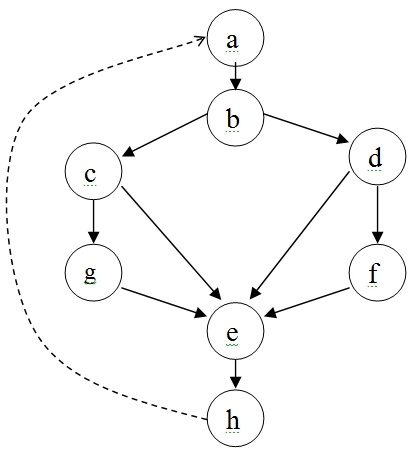
\includegraphics[width=10cm]{metrics_Mackkaib_1.jpg}
    \caption{граф в метриці Маккейба}
    \label{fig:awesome_image}
\end{figure}

Для програми цикломатичне число при l = 10, v = 8, n = 1 визначиться як Z ( G) = 10-8 +2 = 4 .

Таким чином, є Сільносвязанная граф з чотирма лінійно незалежними контурами :

a - b - c - g - e - h - a ;

a - b - c - e - h - a ;

a - b - d - f - e - h - a ;

a - b - d - e - h - a ;

Розглянемо метрику складності програми, що отримала назву « підрахунок точок перетину «, авторами якої є М Вудвард, М Хенель і Д Хидли . Метрика орієнтована на аналіз програм, при створенні яких використовувалося неструктурні кодування на таких мовах, як мова асемблера і фортран . Вводячи цю метрику, її автори прагнули оцінити взаємозв'язку між фізичними місцеположеннями керуючих переходів .

Структурний кодування припускає використання обмеженого безлічі керуючих структур в якості первинних елементів будь-якої програми . У класичному структурному кодуванні, що базується на роботах професора Ейндховенського технологічного університету ( Нідерланди ) Е. Дейкстри, оперують тільки трьома такими структурами : проходженням операторів, розвилкою з операторів, циклом над оператором. всі ці різновиди зображуються найпростішими планарними графами програм. За правилами структурного кодування будь-яка програма складається шляхом вибудовування ланцюжків з 3х згаданих структур або приміщення однієї структури в іншу. Ці операції не порушують планарности графа всієї програми .

У графі програми, де кожному оператору відповідає вершина, тобто не виключені лінійні ділянки, при передачі управління від вершини a до b номер оператора a дорівнює min ( a, b ), а номер оператора b - max ( a, b ) . Тоді перетин дуг з'являться, якщо

min ( a, b ) \textless{} min ( p, q ) \textless{} max ( a, b ) \& max ( p, q ) \textgreater{} max ( a, b ) \textbar{}

\begin{list}{0em}
\item[] Min ( a, b ) \textless{} max ( p, q ) \textless{} max ( a, b ) \& min ( p, q ) \textless{} min ( a, b ) .
\end{list}

Іншими словами, точка перетину дуг виникає у разі виходу управління за межі пари вершин ( a, b ) .

Кількість точок перетину дуг графа програми дає характеристику неструктурованості програми.


\subsection{Метрика Джилба}
\label{2section:id12}
Однією з найбільш простих, але досить ефективних оцінок складності програм є метрика Т. Джілбі, в якій логічна складність програми визначається як насиченість програми виразами IF\_THEN\_ELSE . При цьому вводяться дві характеристики :

СL - абсолютна складність програми, що характеризується кількістю операторів умови;
cl - відносна складність програми, що характеризується насиченістю програми операторами умови, тобто cl визначається як відношення CL до загального числа операторів.
Використовуючи метрику Джілбі, її доповнили ще однією складовою, а саме характеристикою максимального рівня вкладеності оператора CLI, що дозволило застосувати метрику Джілбі до аналізу циклічних конструкцій.

Великий інтерес представляє оцінка складності програм за методом граничних значень .

Введемо кілька додаткових понять, пов'язаних з графом програми .

Нехай G = (V, E) - орієнтований граф програми з єдиною початковою і єдиною окнечной вершинами. У цьому графі число входять до вершину дуг називається негативною ступенем вершини, а число що виходять з вершини дуг - позитивної ступенем вершини . Тоді набір вершин графа можна розбити на дві групи:

вершини у яких позитивна ступінь \textless{}= 1 ;
вершини у яких позитивна ступінь \textgreater{} = 2 .
Вершини першої групи назвемо приймаючими вершинами, а вершини другої групи - вершинами відбору.

Для отримання оцінки за методом граничних значень необхідно розбити

граф G на максимальне число подграфов G `, що задовольняють таким умовам:

вхід в подграф здійснюється тільки через вершину відбору;
кожен подграф включає вершину ( звану нижньою межею подграфа ), в яку можна потрапити з будь-якої іншої вершини подграфа . Наприклад, вершина відбору поєднана сама з собою дугою петлею, утворює подграф .

\begin{figure}
    \centering
    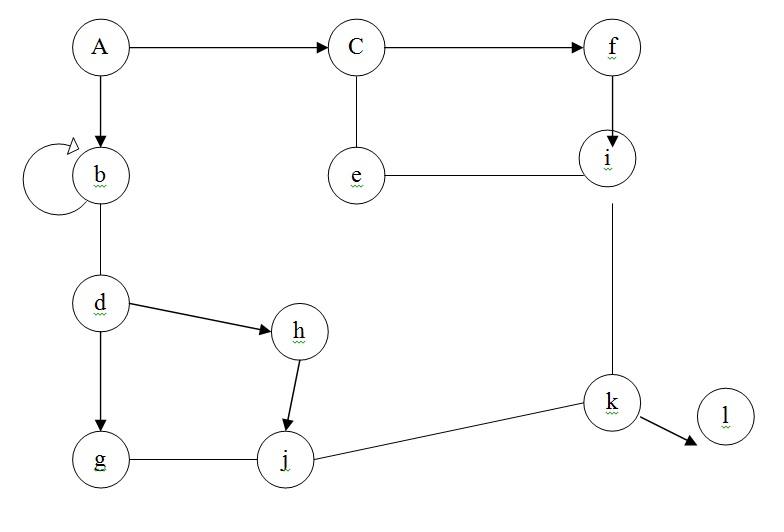
\includegraphics[width=10cm]{metrics_Jilb_1.jpg}
    \caption{граф в метриці Джилба}
    \label{fig:awesome_image}
\end{figure}

Число вершин, що утворюють такий подграф, одно скоригованої складності вершини відбору.

Кожна приймаюча вершина має скориговану складність, рівну 1, крім кінцевої вершини, скоригована складність якої дорівнює 0 . Скориговані складності всіх вершин графа G підсумовуються, утворюючи абсолютну граничну складність програми . Після цього визначається відносна гранична складність програми :

S0 = 1 - ( v - 1 ) / Sa,

де S0 - відносна гранична складність програми ; Sa - абсолютна гранична складність програми, v - загальне число вершин графа програми .

Таким чином, відносна складність програми дорівнює

S0 = 1 - ( 11 / 25 ) = 0,56 .

Інша група метрик складності програм - метрика складності потоку даних, тобто використання, конфігурації і розміщення даних в програмах.

Пара « модуль - глобальна змінна» позначається як ( p, r ), де p - модуль, що має доступ до глобальної змінної r . Залежно від наявності в програмі реального обігу до змінної r формуються два типи пар « модуль - глобальна змінна» : фактичні і можливі . Можливе звернення до r за допомогою p показує, що область існування r включає в себе p .

Характеристика Aup говорить про те, скільки разів модулі Up дійсно отримали доступ до глобальних змінних, а число Pup - скільки разів вони могли б отримати доступ.

Відношення числа фактичних звернень до можливих визначається

Rup = Aup / Pup

Ця формула показує наближену ймовірність посилання довільного модуля на довільну глобальну змінну. Очевидно, чим вище ця вірогідність, тим вище ймовірність « несанкціонованого » зміни якої-небудь змінної, що може істотно ускладнити роботи, пов'язані з модифікацією програми .

Покажемо розрахунок метрики « модуль - глобальна змінна» . Нехай у програмі є три глобальні змінні і три підпрограми. Якщо припустити, що кожна підпрограма має доступ до кожної з змінних, то ми отримаємо дев'ять можливих пар, тобто Pup = 9 . Далі нехай першим підпрограма звертається до однієї змінної, другий - двом, а третя не звертається ні до однієї змінної. Тоді Aup = 3, Rup = 3 /9.

Ще одна метрика складності потоку даних - Спен .

Визначення Спен грунтується на локалізації звернення до даних всередині кожної програмної секції.

Спен - це число тверджень, які містять даний ідентифікатор, між його першим і останнім появою в тексті програми . Ідентифікатор, що з'явився n раз, має Спен, рівний n - 1 .

Спен визначає кількість контролюючих тверджень, що вводяться в тіло програми при побудові траси програми з цього ідентифікатором в процесі тестування і налагодження.


\subsection{Алгоритм пошуку залежностей потенційно-небезпечних дефектів програм на основі екстраполяції метричних характеристик вихідних текстів програм для побудови дерева атак}
\label{2section:id13}
Розглянемо програмний продукт в якості множини вразливостей:

$Vuln = {Vuln_1,Vuln_2,....,Vuln_N}$

Маючи вищенаведені характеристики, та множину потенцыйних вразливостей пропоную створити наступну модель вибору потенційно небезпечних дефектів реакції програм для кібернетичного впливу:

$P_{Vuln_i} = \frac{V_i Z(G)_i}{Z(G) \frac{V}{C_v}}Rup_i, де$
\begin{itemize}
\item {} 
V - Обсяг програми

\item {} 
Vi - обсяг підпрограми

\item {} 
Cv - кікькість потенційних вразливостей

\item {} 
Z(G)i - цикломатична складність підпрограми, в якій знаходиться дефект

\item {} 
Z(G) - цикломатична складність всього коду досліджуваного проекту

\item {} 
Rup - кількість звернень потенційно-вразливої ділянки коду до глобальних змінних

\end{itemize}
\begin{description}
\item[{Розглянемо кожну властивість поданих метрик в контексті відображення наявності можливості використання дефекту переповнення буферу:}] \leavevmode\begin{itemize}
\item {} 
Обсяг програми - обсяг програми напряму впливає на кількість помилок в ній

\item {} 
Аналогічним чиним від обсягу підпрограми, в якій знаходиться потенційна вразливість залежить можливість її використання

\item {} 
Від цикломатичної складності залежить наскільки просто буде проаналізувати логіку коду і швидко розібратись, як саме можна використати дефект

\item {} 
А від кількості звернень до потенційно-вразливої ділянки коду можна зробити висновок, як локальні дані між собою звязані і чи можливо здійснити вплив на певні управляючі дані через суміжні

\end{itemize}

\end{description}

Дана ймовірність буде наближеною та неточною, але якщо набір таких ймовірностей збільшувати і розглянути їх як протабульовану функцію
$f(V,V_i,C_v,Z(G)_i,Z(G),Rup) = P_{vuln_i}$
то можна спробувати робити прогноз наявності вразливих ділянок при аналізі нового вихідного тексту на основі  його метрик коду - що дозволить побудувати ефективне дерево атак.


\subsection{Дерева атак}
\label{2section:id14}
Дерева атак - це діаграми, що демонструють, як може бути атакована мету. Дерева атак використовуються в безлічі областей. В області інформаційних технологій вони застосовуються, щоб описати потенційні загрози комп'ютерній системі і можливі способи атаки, реалізують ці загрози. Однак, їх використання не обмежується аналізом звичайних інформаційних систем. Вони також широко використовуються в авіації і обороні для аналізу ймовірних загроз, пов'язаних зі стійкими до спотворень електронними системами. (Наприклад на авіонику військових літальних засобів).

Збільшується застосування дерев атак в комп'ютерних системах контролю (особливо пов'язаних з енергетичними мережами). {[}2{]} Також дерева атаки використовуються для розуміння загроз, пов'язаних з фізичними системами.

Деякі з найбільш ранніх описів дерев атак знайдені в доповідях і статтях Брюса Шнайера {[}3{]}, технічного директора Counterpane Internet Security. Шнайер був безпосередньо залучений в розробку концептуальної моделі дерев атаки і зіграв важливу роль в її поширенні. Тим не менш, в деяких ранніх опублікованих статтях по деревах атак {[}4{]} висловлюються припущення про залученість Агентства Національної Безпеки в початковий етап розробки.

Дерева атак дуже схожі на дерева загроз. Дерева загроз були розглянуті в 1994 роки Едвардом Аморосо. {[}5{]}

Дерева атак це мультирівневих діаграми, що складаються з одного кореня, листя і нащадків. Будемо розглядати вузли знизу вгору. Дочірні вузли це умови, які повинні виконуватися, щоб батьківський вузол також перейшов в справжній стан. Коли корінь переходить у справжній стан, атака успішно завершена. Кожен вузол може бути приведений у справжній стан тільки його прямими нащадками.

Вузол може бути дочірнім для іншого вузла, в цьому випадку, логічно, що для успіху атаки потрібно кілька кроків. Наприклад, уявіть клас з комп'ютерами, де комп'ютери прикріплені до парт. Щоб вкрасти один з них необхідно або перерізати кріплення, або відкрити замок. Замок можна відкрити відмичкою або ключем. Ключ можна отримати шляхом погроз його власнику, через підкуп власника або ж просто вкрасти його. Таким чином, можна намалювати чотирирівневої дерево атаки, де одним із шляхів буде: Підкуп власника ключа-Отримання ключа-Відмикання замку-Винос комп'ютера.

Також слід враховувати, що атака, описана у вузлі може зажадати, щоб одна або декілька з безлічі атак, описаних в дочірніх вузлах були успішно проведені. Вище ми показали дерево атаки тільки зі зв'язком типу АБО між нащадками вузла, але умова І також може бути введено, наприклад в класі є електронна сигналізація, яка повинна бути відключена, але тільки в тому випадку, якщо ми вирішимо перерізати кріплення. Замість того, щоб робити відключення сигналізації дочірнім вузлом для перерізання кріплення, обидва завдання можна просто логічно підсумувати, створивши шлях (Відключення сигналізації І Перерізання кріплення)-Винос Комп'ютера.

Дерева атак також пов'язані із створенням дерева помилок. {[}6{]} Метод побудови дерева помилок використовує булеві вирази для створення умов, при яких дочірні вузли забезпечують виконання батьківських вузлів.

Включає апріорні ймовірності в кожен вузол, можливо зробити підрахунок ймовірностей для вузлів, що знаходяться вище по правилу Байеса . Однак, в реальності, точні оцінки ймовірності або недоступні, або занадто дорогі для обчислення. У разі динамічної комп'ютерної безпеки (тобто з урахуванням атакуючих) випадкові події не є незалежними, отже, прямий Байєсівський аналіз не підходить.

Так як Байєсовські аналітичні техніки, що використовуються в аналізі дерев помилок не можуть бути правильно застосовані до дерев атак, аналітики використовують інші техніки {[}7{]} {[}8{]} для визначення яким шляхом піде даний атакуючий. Ці техніки включають порівняння можливостей атакуючого (час, гроші, навички, обладнання) з ресурсами, що вимагаються для даної атаки. Атаки, які вимагають повної віддачі від атакуючого або навіть знаходяться за межами його можливостей куди менш імовірні, ніж дешеві і прості атаки. Ступінь, в якій атака задовольняє цілям атакуючого також впливає на його вибір. З двох можливих атак зазвичай вибирається та, що більшою мірою задовольняє цілям атакуючого.

Дерева атак можуть стати вкрай складними, особливо при розгляді конкретних атак. Повне дерево атаки може містити сотні або тисячі різних шляхів, всі з яких призводять до успіху атаки. Але навіть при такому розкладі, ці дерева вкрай корисні для визначення існуючих загроз і методів їх запобігання.

Дерева атак можуть бути використані для визначення стратегії забезпечення інформаційної безпеки. Також, слід враховувати, що реалізація цієї стратегії сама по собі вносить зміни в дерево атаки. Наприклад, захистом від комп'ютерних вірусів може служити заборона системного адміністратора безпосередньо змінювати існуючі файли і папки, замість цього вимагаючи використання файлового менеджера. Це додає в дерево атаки використання недоліків чи експлойтів файлового менеджера.


\begin{figure}
    \centering
    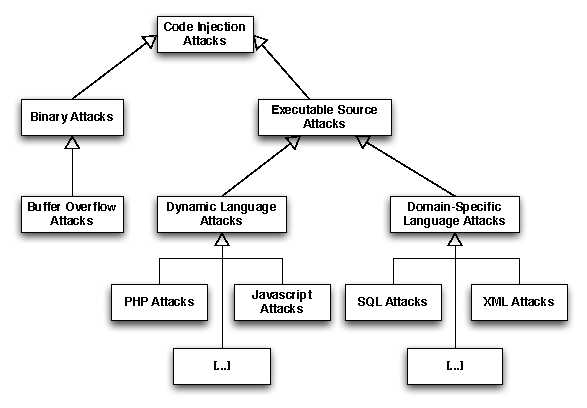
\includegraphics[width=15cm]{attack-tree-uml.png}
    \caption{приклад дерева атак}
    \label{fig:attack_tree_example}
\end{figure}

\section*{Висновки}
\addcontentsline{toc}{section}{Висновки}
Отже,

